\documentclass{standalone}

\usepackage{graphicx}
\usepackage{tikz}

\begin{document}

{\small
\begin{tabular}{ *3{c} }
  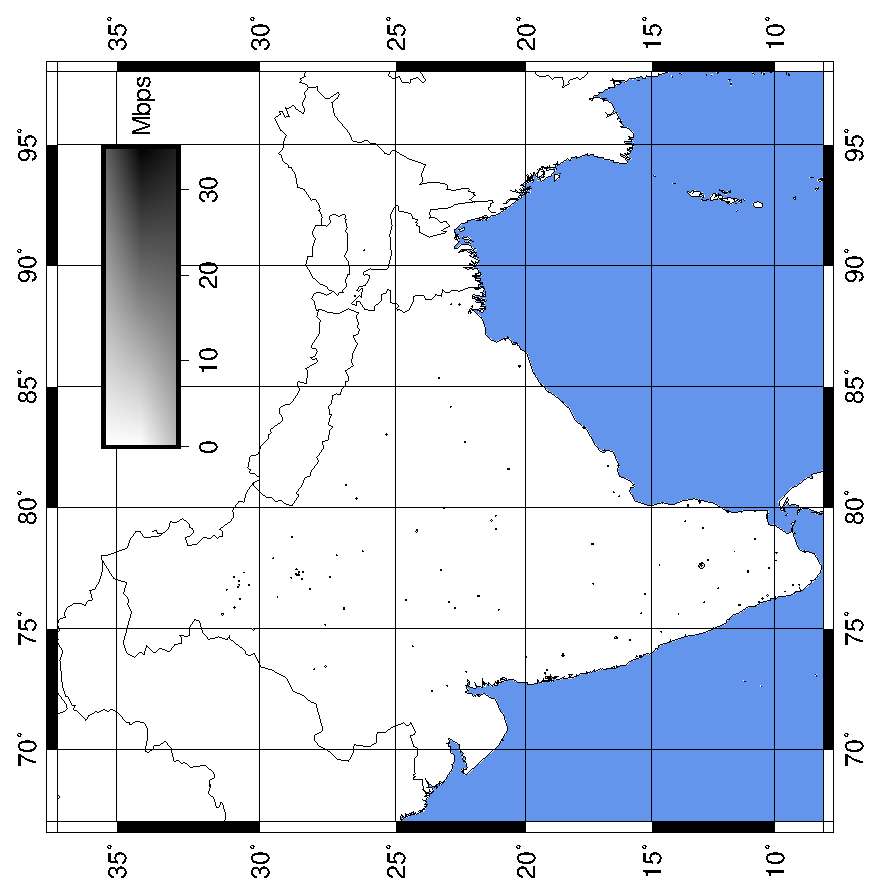
\includegraphics[width=.3\linewidth, angle=270]{2009_09} & 
  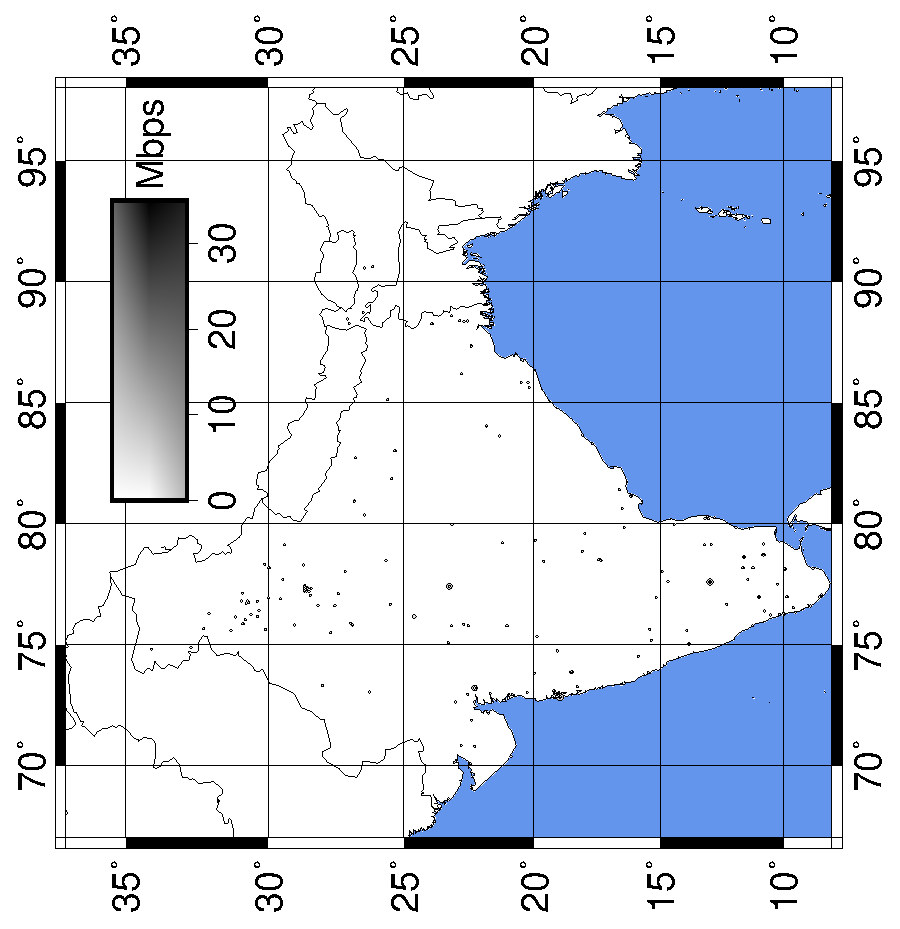
\includegraphics[width=.3\linewidth, angle=270]{2010_09} & 
  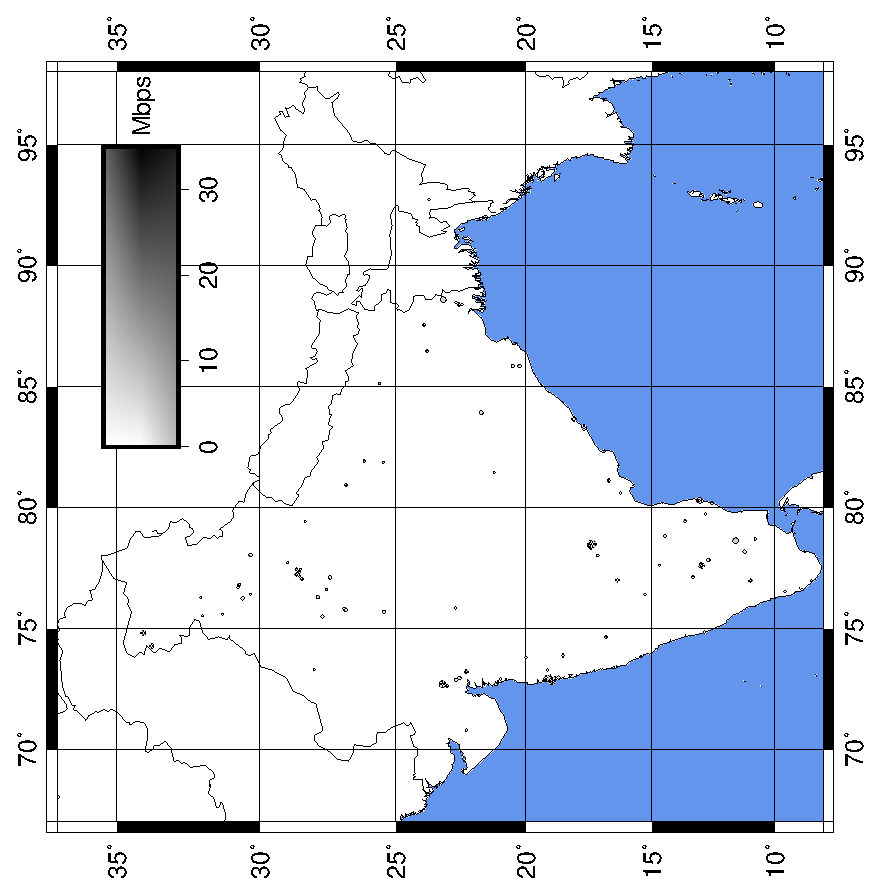
\includegraphics[width=.3\linewidth, angle=270]{2011_09} \\
  (a) September, 2009 & (b) September, 2010 & (c) September, 2011\\
  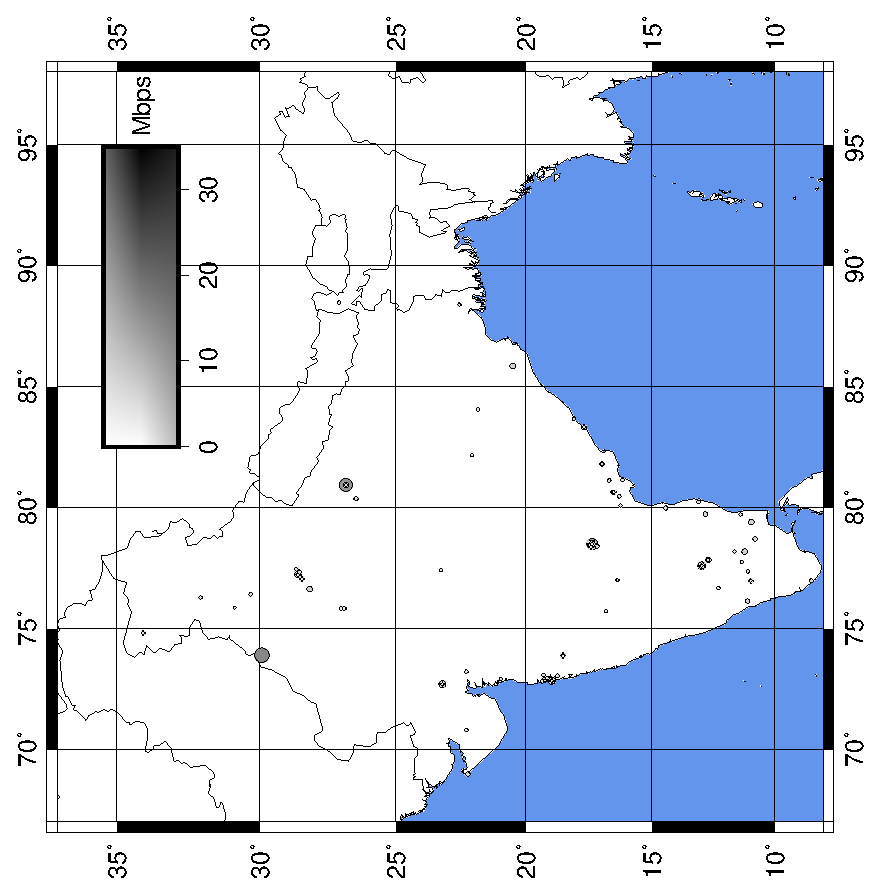
\includegraphics[width=.3\linewidth, angle=270]{2012_09} & 
  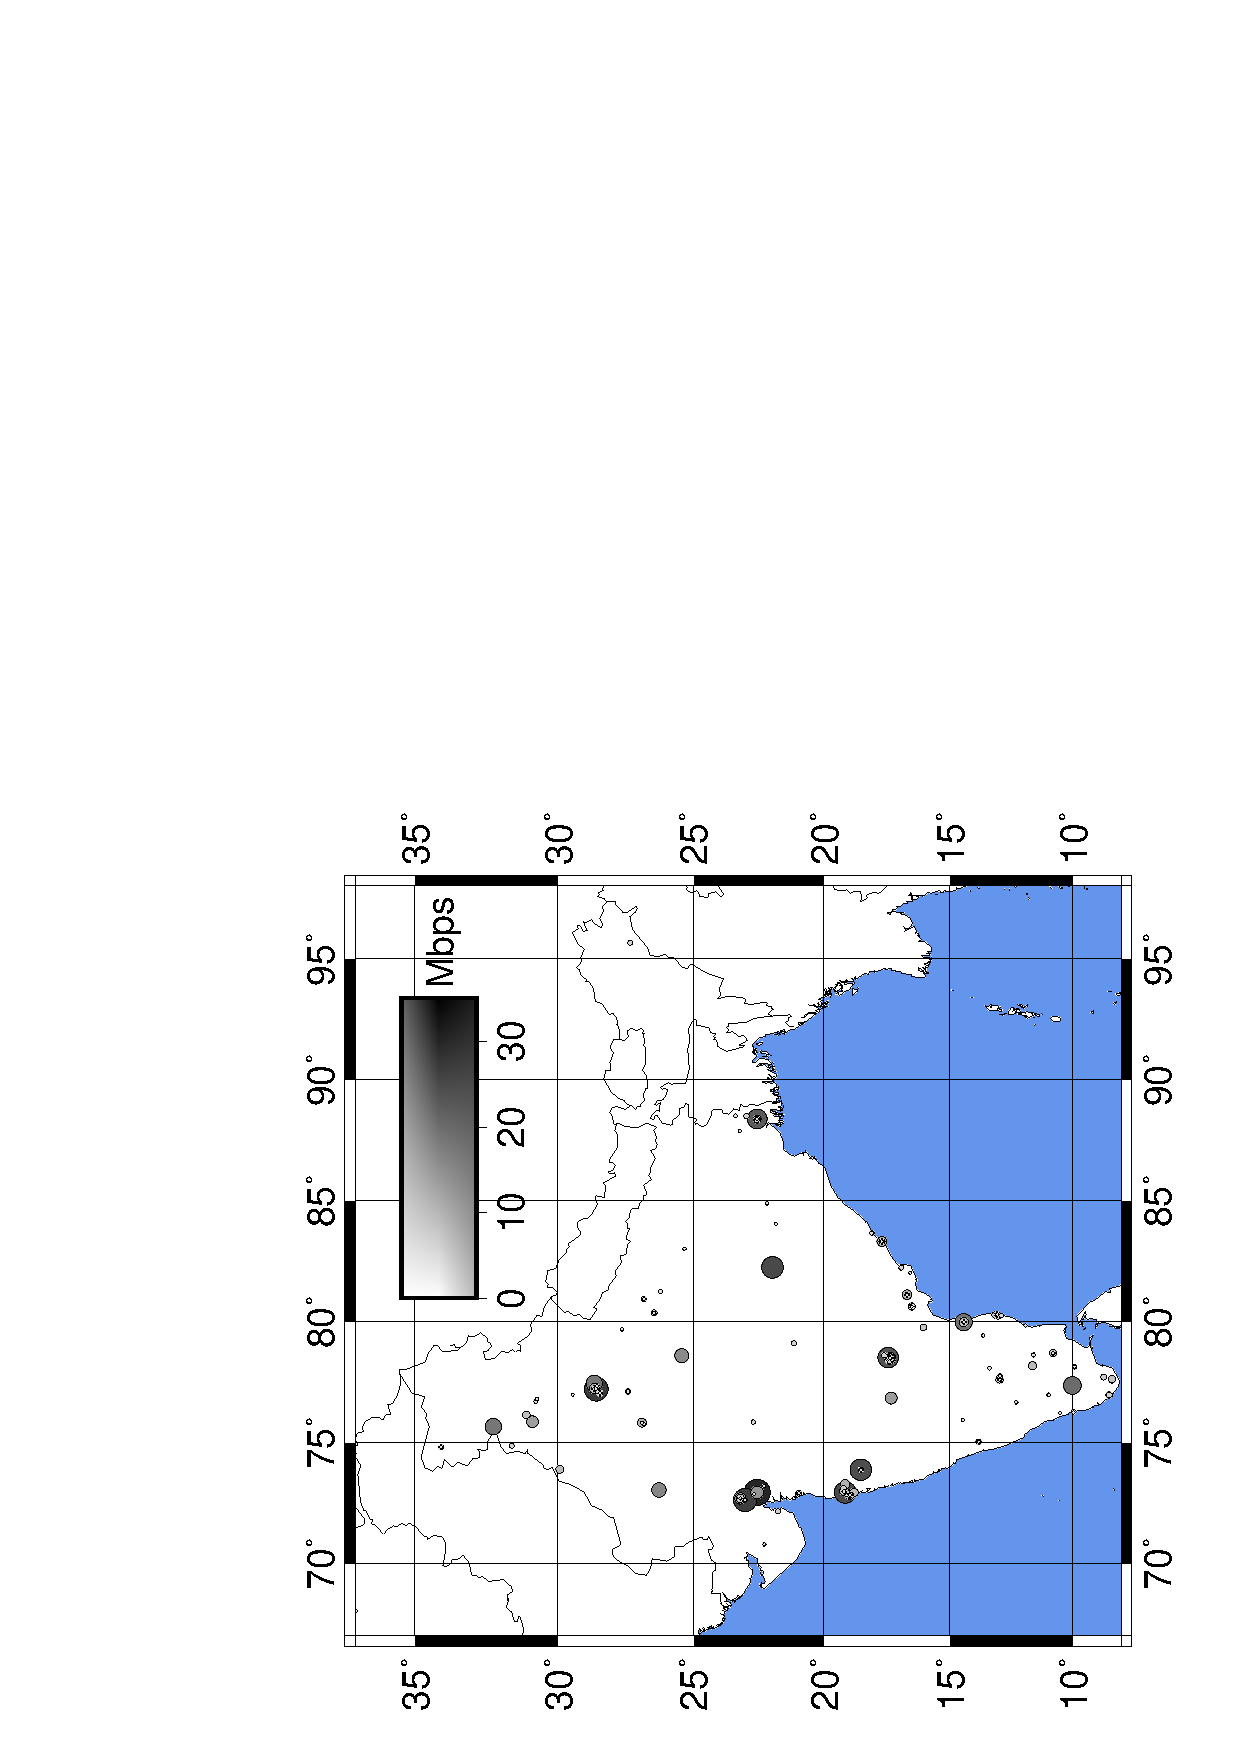
\includegraphics[width=.3\linewidth, angle=270]{2013_09} & 
  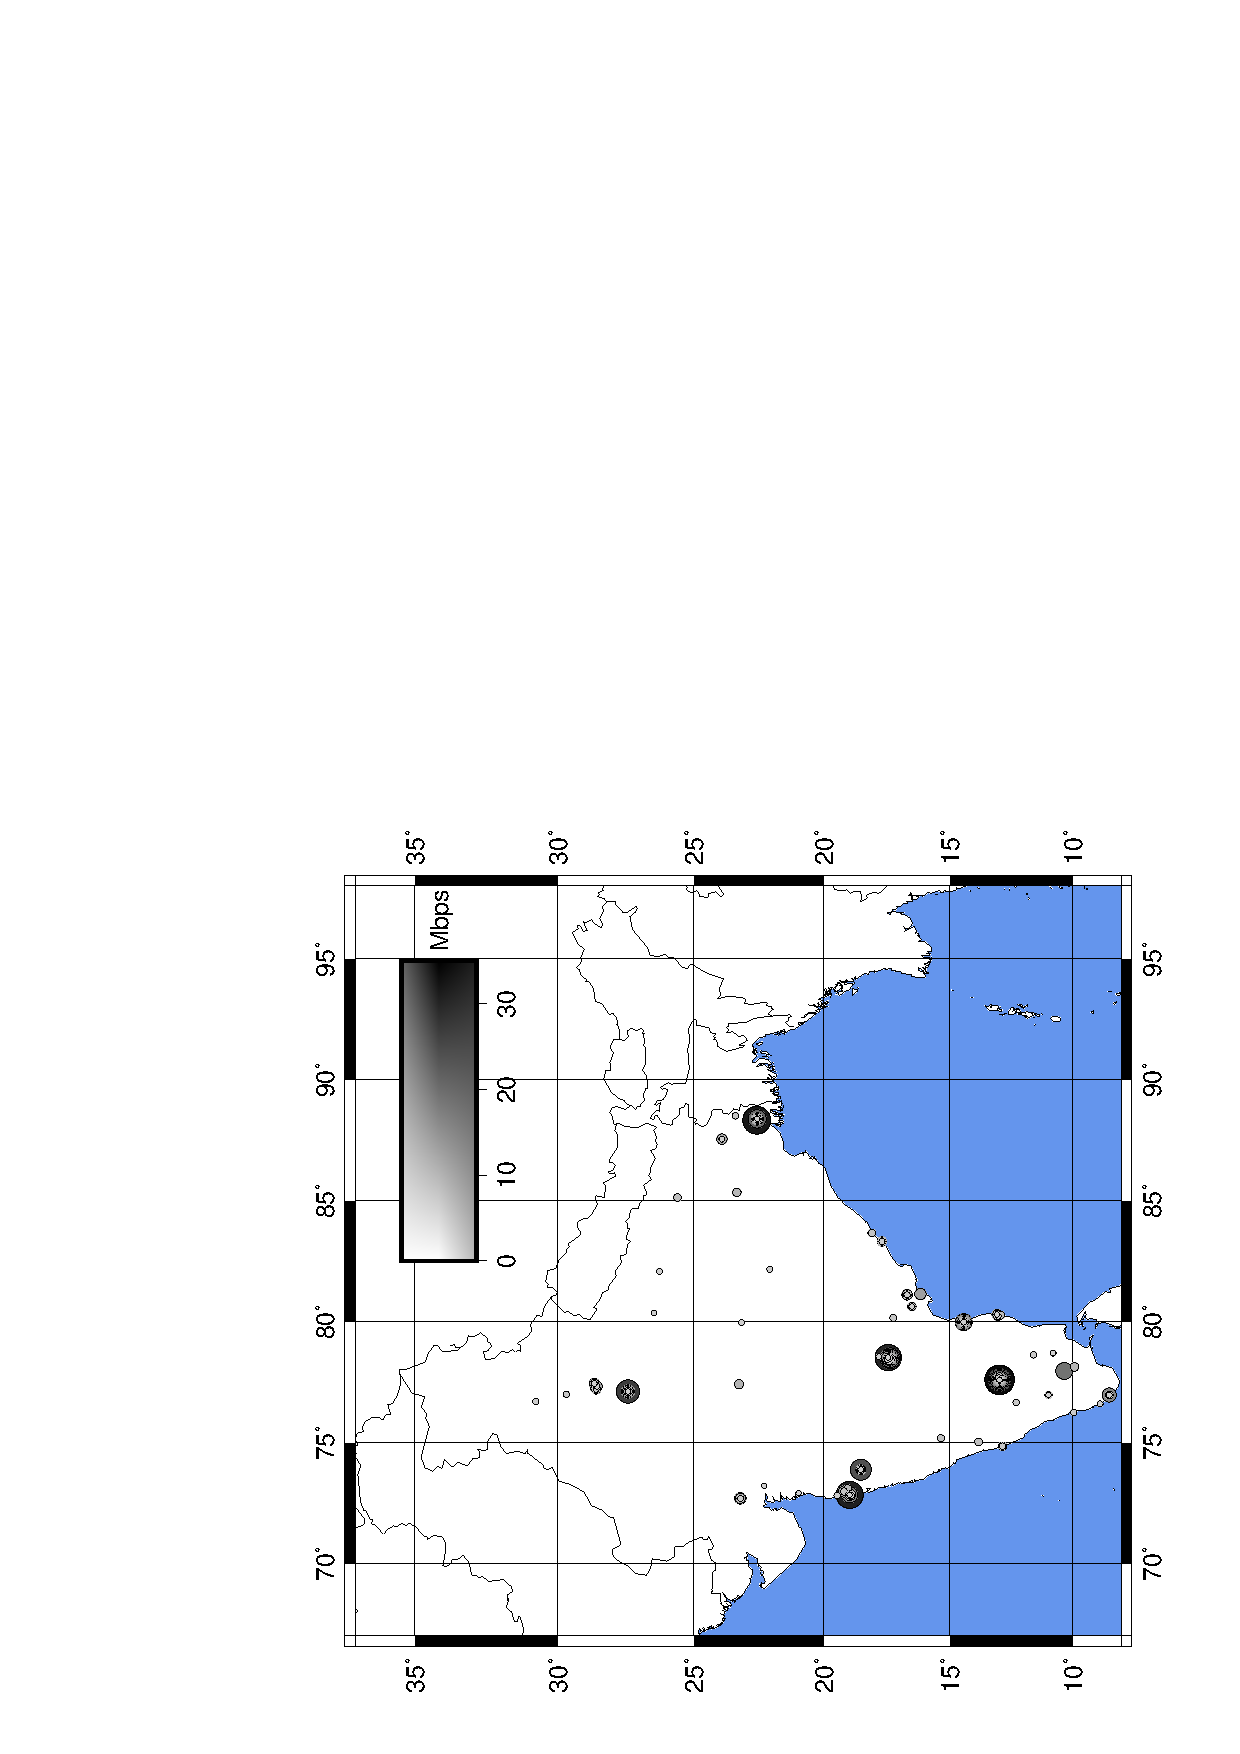
\includegraphics[width=.3\linewidth, angle=270]{2014_09} \\
  (d) September, 2012 & (e) September, 2013 & (f) September, 2014\\
\end{tabular}

}



\begin{tikzpicture}
\node[inner sep=0pt] at (0,0)
    {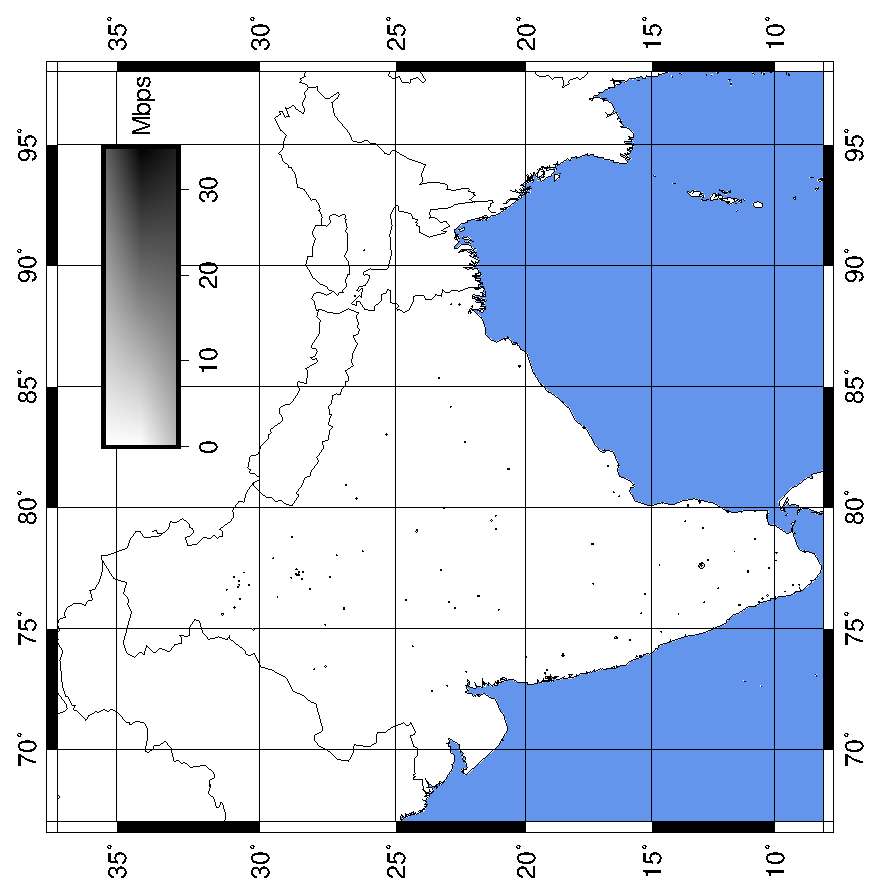
\includegraphics[width=.3\linewidth, angle=270]{2009_09}};
\end{tikzpicture}

\end{document}